\documentclass[runningheads]{llncs}
\usepackage{graphicx}
\usepackage{algorithm}
\usepackage[noend]{algpseudocode}
\usepackage{amsmath}
% New definitions
\algnewcommand\algorithmicswitch{\textbf{switch}}
\algnewcommand\algorithmiccase{\textbf{case}}
\algnewcommand\algorithmicotherwise{\textbf{otherwise}}
\algnewcommand\algorithmicassert{\texttt{assert}}
\algnewcommand\Assert[1]{\State \algorithmicassert(#1)}%
% New "environments"
\algdef{SE}[SWITCH]{Switch}{EndSwitch}[1]{\algorithmicswitch\ #1\ \algorithmicdo}{\algorithmicend\ \algorithmicswitch}%
\algdef{SE}[CASE]{Case}{EndCase}[1]{\algorithmiccase\ #1}{\algorithmicend\ \algorithmiccase}%
\algdef{SE}[CASE]{Otherwise}{EndOtherwise}[1]{\algorithmicotherwise\ #1}{\algorithmicend\ \algorithmicotherwise}%
\algtext*{EndSwitch}%
\algtext*{EndCase}%
\algtext*{EndOtherwise}%
\usepackage{tabularx}
\usepackage{array}
\newcommand{\tabincell}[2]{\begin{tabular}{@{}#1@{}}#2\end{tabular}}














\begin{document}
\title{Verifying Strong Ground Bisimilarity of Quantum Programs}
\author{First Author\inst{1} \and
Second Author\inst{2,3} \and
Third Author\inst{3}}

\authorrunning{}

\institute{University, Princeton NJ 08544, USA \and
Springer Heidelberg, Tiergartenstr. 17, 69121 Heidelberg, Germany
\email{lncs@springer.com}\\
\url{http://www.springer.com/gp/computer-science/lncs} \and
ABC Institute, Rupert-Karls-University Heidelberg, Heidelberg, Germany\\
\email{\{abc,lncs\}@uni-heidelberg.de}}

\maketitle

\begin{abstract}Several bisimulations on quantum processes have been proposed. The symbolic quantum bisimulation is proposed for verifying programs with arbitrary iuput values, its ``concrete'' version still needs input but does not have problem on normalizing measurement result. This paper gives a strong ground bisimulation verification algorithm for quantum programs basing on the ``concrete'' version of quantum bisimulation. Furthermore, we implement the algorithm that enable us to make experiments on existing quantum communication protocols. As a preparation of the experiments, we encode the quantum communication protocol into a quantum program. Then we check whether a quantum program is bisimilar with its specification. According to the results, we make some improvements on the quantum programs.

\keywords{Quantum programs  \and Verification \and Bisimualtion.}
\end{abstract}

\section{Introduction}

\section{Preliminaries}

\section{qCCS}

\section{Bisimulation Verification}
In this section, we give an algorithm to verify the strong ground bisimulation.

\begin{algorithm}[h]
\caption{Bisim(t,u)}
\label{alg:bisim}
\begin{algorithmic}[1]
\Require A pair of initial states for matching $t$,$u$.
\Ensure A boolean value $\theta$ showing if two pLTSs are bisimilar and a set of non-bisimilar state pairs $N$.
\Function{\textbf{Bisim}}{$t,u$}
\State \textbf{return} \textbf{Match}(\textit{t,u,W})
\EndFunction
\State
\Function{\textbf{Match}}{$t,u,W$}\Comment{$t=\langle t,\rho\rangle\ and\ u=\langle u,\sigma\rangle$}
\If{$t,u\in W$}
    \State $\theta:=\texttt{tt}$
\Else
    \For{$\gamma\in \texttt{Act}(t,u)$}
        \State ($\theta_{\gamma} ,N_{\gamma}$):=\textbf{MatchAction}(\textit{$\gamma$,t,u,W})
    \EndFor
    \State $\theta$:=$\bigwedge_\gamma\theta_\gamma\wedge qv(t)=qv(u)\wedge tr_{\overline{qv(t)}}(\rho)=tr_{\overline{qv(t)}}(\sigma)$
    \State $N=\bigcup_{\gamma}N_\gamma$
    \If{$\theta=\texttt{ff}$} $N$:=$N\cup \{(t,u)\}$ \EndIf
\EndIf
\State \textbf{return} ($\theta,N$) 
\EndFunction
\State
\Function{\textbf{MatchAction}}{$\gamma,t,u,W$}
\Switch{$\gamma$}
\Case{$c!$}
\For{$t\xrightarrow{c!e_i}t_i \text{ and } u\xrightarrow{c!e'_j}u_j$}
    \State $(\theta_{ij},N_{ij}):=\textbf{Match}(t_i,u_j,W\cup \{(t,u)\}$
\EndFor
\State \textbf{return} $(\bigwedge_{i}(\bigvee_j(\theta_{ij}\wedge e_i=e'_j))\wedge\bigwedge_{j}(\bigvee_i(\theta_{ij}\wedge e_i=e'_j)),\bigcup_{ij}N_{ij})$
\EndCase
\Case{$\tau$}
\For{$t\xrightarrow{\tau}\Delta_i \text{ and } u\xrightarrow{\tau}\Theta_j$}
    \State $(\theta_{ij},N_{ij}):=\textbf{MatchDistribution}(\Delta_i,\Theta_j,W\cup \{(t,u)\}$
\EndFor
\State \textbf{return} $(\bigwedge_{i}(\bigvee_j\theta_{ij})\wedge\bigwedge_{j}(\bigvee_i\theta_{ij}),\bigcup_{ij}N_{ij})$
\EndCase
\Otherwise{}
\For{$t\xrightarrow{\gamma}t_i \text{ and } u\xrightarrow{\gamma}u_j$}
    \State $(\theta_{ij},N_{ij}):=\textbf{Match}(t_i,u_j,W\cup \{(t,u)\}$
\EndFor
\State \textbf{return} $(\bigwedge_{i}(\bigvee_j\theta_{ij})\wedge\bigwedge_{j}(\bigvee_i\theta_{ij}),\bigcup_{ij}N_{ij})$
\EndOtherwise
\EndSwitch
\EndFunction
\State
\Function{\textbf{MatchDistribution}}{$\Delta,\Theta,W$}
\For{$t_i\in \lceil\Delta\rceil\text{ and }u_j\in \lceil\Theta\rceil$}
    \State $(\theta_{ij},N_{ij}):=\textbf{Match}(t_i,u_j,W)$
\EndFor
\State $\textit{R}$:=$\{(t_i,u_j)|(t_i,u_j)\notin \bigcup_{ij}N_{ij}\}*$
\State \textbf{return} ($\textbf{Check}(\textit{$\Delta$,$\Theta$,$R$})\wedge\bigvee_{ij}\theta_{ij},\bigcup_{ij}N_{ij}$)
\EndFunction
% \State
% \Function{\textbf{Check}}{$\Delta,\Theta,\textit{R}$}
% \EndFunction
\end{algorithmic}
\end{algorithm}

The algorithm~\ref{alg:bisim} bases on the work of \cite{TOCL2014}. The main function is \textbf{Bisim}$(t,u)$, its job is to initialize the start states pair $(t,u)$, visited states pair $W$ which is an empty set and then find the bisimulation basing on that initialization. The difference between it and the previous work in several aspects.

The algorithm keeps updating two sets, $W$ for visited state pairs and $N$ for non-bisimilar state pairs. The function \textbf{Match}$(t,u,W)$ invokes a depth-first traversal to match a pair of 
states $(t,u)$ with all their possible behaviors. The state pair will be non-bisimilar if one of their transitions are not matched or their quantum variables are not matched, so do the quantum registers. All the non-bisimilar state pairs are added into $N$. 

An auxiliary function \textbf{Act}$(t,u)$ is called in \textbf{Match} to discover the next action that both two states can behave. If both of two states have no more action to do it returns an empty set. In addition, if only one of them has no more action to do that will lead to a non-bisimilarity. It makes the algorithm more efficient as it terminates at an early time point if those pLTSs are indeed not bisimilar. Next we prove why we can ensure that.
\begin{lemma}
Todo: prove that we can ensure in such case, the trace is  longer than any other trace from another side or unmatched with them.
\end{lemma}
\begin{theorem}[Early termination]
If the algorithm reaches a leaf state of the tree-like pLTS while the state of the other pLTS is not a leaf state, then these two pLTSs are not bisimilar.
\end{theorem}
\begin{proof}
We consider it on the aspect of the length of the traces. From the structure of the algorithm, each time \textbf{MatchAction} is called \textbf{Act} will be called before it. So we can ensure that two states have the same action to behave. There exists the trace that
\[T = \langle t_0,\rho\rangle\xrightarrow{\gamma_0}...\xrightarrow{\gamma_i}\langle t_i,\rho\rangle\text{ and }U = \langle u_0,\sigma\rangle\xrightarrow{\gamma_0}...\xrightarrow{\gamma_i}\langle u_i,\sigma\rangle.\]
Let $|T|=|U|=n$, if one of these states $u_i$ is not a leaf, then there has a longer trace $|U'|=n+1$. As there is no loop contained, the trace $|T'|=n+1$ does not exist, so we can not find a trace has the same length as that one. According to the definition of the bisimulation, these two pLTS should not satisfy it.
\end{proof}

The other set $W$ is updated in \textbf{MatchAction}$(\gamma,t,u,W)$. It discovers next state pairs according to the action $\gamma$ and recursively invokes the function \textbf{Match} when there is a pair of states or \textbf{MatchDistribution} when there is a pair of state distributions. The current state pair is added to $W$ when the new function is invoked.

The \textbf{MatchDistribution}$(\Delta,\Theta,\textit{R})$ is an extra step between \textbf{Match} and \textbf{MatchAction} if we match a pair of state distributions instead of a single pair of states. It returns a boolean value indicating if the distributions are bisimilar. It matches each pair of states from the distributions. After checking the bisimilarity of these state pairs, the function generates an equivalence relation of the state pairs those who are not contained in the non-bisimilar state pairs set $N$. Another auxiliary function \textbf{Check}$(\Delta,\Theta,\textit{R})$ is used for checking the lifting condition of the bisimulation relation. Besides the lifting condition, we check the disjunction of the returning boolean value from \textbf{Match} functions. The function returns such result basing on the following definition.

\begin{definition}[Lifting Condition]

Let $\textit{R}\subseteq Dist(Con)\times Dist(Con)$ be the (strong) open bisimulation relation between two distributions, then for any $\mu,\nu\in Dist(Con),\ \mu\textit{R}\nu$ can imply that:
\begin{item}
\item[(1)] The relation satisfies the lifting condition, that is $\mu=\sum_{i\in I}p_i\textit{C}_i$, for each $i\in I,\ \textit{C}_i\textit{R}\textit{D}_i$ for some $\textit{D}_i$, and $\nu=\sum_{i\in I}p_i\textit{D}_i$.
\item[(2)] The set $I$ is not an empty set, s.t. $\exists C,D\in Con, \mu(C)>0\wedge\nu(D)>0$.
\end{item}
\end{definition}
After the introduction of the algorithm, we discuss its termination and correctness. They are presented in the theorem below.
\begin{theorem}[Termination]

Given two states $t$ and $u$ from two pLTSs, \textbf{Bisim(t,u)} always terminates.
\end{theorem} 
\begin{proof}
So far there is no while-loop in the qCCS, that brings convenience to the proof of termination. Starting at the initial pair of states, the next action to do will be detected in the function \textbf{Match}. Then it invokes function \textbf{MatchAction} to find the next new pair of states and recursively call function \textbf{Match} to check them. Each time function \textbf{MatchAction} calls function \textbf{Match} it adds the current states pair into $W$ at the same time. If we reach the leaf nodes, there is no more action, we only compare the quantum variables used and the state of quantum registers. After that, the function terminates, so do the calls to the other functions. Moreover, if there still exists actions to do in one of the pLTS while another one does not, that means they are not strong bisimilar and then the whole algorithm terminates. 
\end{proof}
Then we consider the correctness of the algorithm. First, we let $(\theta, N)$ to be the return pair of functions, moreover $(\theta_{ij}, N_{ij})$ is the return of the $i\cdot j$-th execution of the function. To simplify the explanation, we use \texttt{R}$(t,u,W,N)$ to mean the following condition is satisfied:

If $(t',u')\in N$, then $\forall t'\xrightarrow{\alpha}t'',u'\xrightarrow{\alpha'}u'',\ t''\not\sim u''$. 

If $(t',u')\notin N$, then $\forall t'\xrightarrow{\alpha}t'',\exists u'\xrightarrow{\alpha'}u''$ and $(t'',u'')\notin \{(t,u)\}\cup W$ such that: 
\begin{itemize}
    \item if $\alpha\equiv a$ (including $c?x$) then $\alpha'\equiv a$ and $(t'',u'')\notin W\wedge(t'',u'')\notin N\implies t''\sim u''$.
    \item if $\alpha\equiv c!e$ then $\alpha'\equiv c!e'$ with $e=e'$ and $(t'',u'')\notin W\wedge(t'',u'')\notin N\implies t''\sim u''$.
    \item let $t''\equiv \Delta'$ and $u''\equiv \Theta'$, if $\alpha\equiv \tau$ then $\alpha'\equiv \tau$, $\forall t'_i\in \lceil\Delta'\rceil, u'_j\in \lceil\Theta'\rceil,\ (t'_i,u'_j)\notin W\wedge(t'_i,u'_j)\notin N\implies t'_i\sim u'_j$.
\end{itemize}

We define the verification conditions of our three matching functions.
\begin{definition}\label{def:match}
\textbf{Match}$(t,u,W)$ is \textit{true} if the following condition is satisfied:
\begin{itemize}
    \item(C1) $W\cap N=\emptyset$.
    \item(C2) if $(t,u)\in W$, then $(t,u)\notin N$.
    \item(C3) if $(t,u)\notin W$, then either $\theta=true\wedge(t,u)\notin N$ or $\theta=false\wedge(t,u)\in N$.
    \item(C4) $\texttt{R}(t,u,W,N)$.
\end{itemize}
Let \textbf{Bisim}$(t,u)=$\textbf{Match}$(t,u,\emptyset)$.
\end{definition}
\begin{definition}\label{def:matchaction}
\textbf{MatchAction}$(\gamma,t,u,W)$ is \textit{true} if the following conditions are satisfied:
\begin{itemize}
    \item(M1) $W\cap N=\emptyset$, $(t,u)\notin W$ and $(t,u)\notin N$.
    \item(M2) $\texttt{R}(t,u,W,N)$.
    \item(M3) $\forall t\xrightarrow{\alpha}t', \exists u\xrightarrow{\alpha'}u'$, $(t',u')\notin \{(t,u)\}\cup W$ and 
    \begin{itemize}
        \item if $\alpha\equiv a$ (including $c?x$) then $\alpha'\equiv a$ and $(t',u')\notin W\wedge(t',u')\notin N\implies t'\sim u'$.
        \item if $\alpha\equiv c!e$ then $\alpha'\equiv c!e'$ with $e=e'$ and $(t',u')\notin W\wedge(t',u')\notin N\implies t'\sim u'$.
        \item let $t'\equiv \Delta$ and $u'\equiv \Theta$, if $\alpha\equiv \tau$ then $\alpha'\equiv \tau$, $\forall t_i\in \lceil\Delta\rceil, u_j\in \lceil\Theta\rceil,\ (t_i,u_j)\notin W\wedge(t_i,u_j)\notin N\implies t_i\sim u_j$.
    \end{itemize}
\end{itemize}
\end{definition}
\begin{definition}\label{def:matchdistribution}
\textbf{MatchDistribution}$(\Delta,\Theta,W)$ is \textit{true} if the following conditions are satisfied:
\begin{itemize}
    \item(D1) $W\cap N=\emptyset$, $\forall t_i\in \lceil\Delta\rceil, u_j\in \lceil\Theta\rceil,\ (t_i,u_j)\notin W$.
    % and $(t_i,u_j)\notin N\implies t_i\sim u_j$
    \item(D2) Let $t\xrightarrow{\alpha}\Delta, u\xrightarrow{\alpha'}\Theta$, $\texttt{R}(t,u,W,N)$.
\end{itemize}
\end{definition}
\begin{proposition}Let $\textbf{MatchAction}_\gamma(\gamma,t,u,W)$ is the execution of the function with action $\gamma$.
If $\textbf{MatchAction}_\gamma(\gamma,t,u,W)$ is $true$ for each action $\gamma$ then \textbf{Match}$(t,u,W)$ is also $true$, where it returns $\theta=\bigwedge_\gamma\theta_\gamma$ and $N=\bigcup_\gamma N_\gamma$.
\end{proposition}
\begin{proof}
As $(t,u)$ is added into $W$ during the execution of \textbf{MatchAction}, according to the Definition~\ref{def:matchaction}, $W\cap N=\emptyset$. 

$(t,u)\notin N_{\gamma}$ implies that $(t,u)\notin N=\bigcup_{\gamma} N_{\gamma}$. $(t,u)$ will be added into $N$ if $\theta=\wedge_{\gamma}\theta_{\gamma}$ is $false$. Since the verified pLTS is a finite tree, if they reach the leaf states of the pLTSs, there should be $\theta=true$ and $N=\emptyset$, at the same time it satisfies that $(t,u)\notin W\wedge(t,u)\notin N$. 

So it satisfies the verifying condition of \textbf{Match}.
\end{proof}
\begin{proposition} Suppose $(t,u)\notin W$.
If \textbf{Match}$(t_i,u_j,W\cup\{(t,u)\})$ is $true$ for all action $\gamma\neq\tau$ derivations$(t\xrightarrow{\gamma}t_i$, $u\xrightarrow{\gamma}u_j)$ or \textbf{MatchDistribution}$(\Delta_i,\Theta_j,W\cup\{(t,u)\})$ is $true$ for all action $\gamma=\tau$ derivations $(t\xrightarrow{\tau}\Delta_i,u\xrightarrow{\tau}\Theta_j)$ then\\
\textbf{MatchAction}$(\gamma,t,u,W\cup\{(t,u)\})$ is $true$ where
$\theta=\bigwedge_i(\bigvee_j\theta_{ij})\wedge\bigwedge_j(\bigvee_i\theta_{ij})$, $N=\bigcup N_{ij}$.
\end{proposition}
\begin{proof}
From the structure of the function \textbf{MatchAction}, the first condition is satisfied.

To show M2 and M3, we first consider the case where $(t_i,u_j)$ is already the leaf of the finite tree, and if $\theta_{ij}=qv(t_i)=qv(u_j)\wedge(tr_{\overline{qv(u_i)}}\rho_i)=tr_{\overline{qv(u_j)}}(\sigma_j)$ is $true$, $(t_i,u_j)\notin N_{ij}$ and $t_i\sim u_j$. 

If it is not the leaf node, by (C4), we have \texttt{R}$(t_i,u_j,\{(t,u)\}\cup W,N_{ij})$. Since 
$\theta=\bigwedge_i(\bigvee_j\theta_{ij})\wedge\bigwedge_j(\bigvee_i\theta_{ij})$ and $N=\bigcup_{ij}N_{ij}$, if $\theta$ is true, there exists $\theta_{ij}$ are $true$, then from $(t_i,u_j)\notin N_{ij}$, we get $(t'_i,u'_j)\notin N_{ij}\implies t'_i\sim u'_j$. In the case $\theta$ is false, $(t,u)\in N$ has already distinguished the non-bisimilarity.

The final case we need consider is the distribution $(\Delta,\Theta)$ instead of a node. If $\theta$ is true, then \textbf{Check} returns $\theta_{ij}$ is also $true$. So there must exist \textbf{Match} returns $true$ implies that $(t_i,u_j)\notin N\implies t_i\sim u_j$.
\end{proof}
\begin{proposition}
Suppose $\forall t_i\in\lceil\Delta\rceil,u_j\in\lceil\Theta\rceil , (t_i,u_j)\notin W$.
If \textbf{Match}$(t_i,u_j,W)$ is $true$ then \textbf{MatchDistribution}$(\Delta,\Theta,W)$ is $true$ where $\Delta$ and $\Theta$ satisfy the condition for lifting condition, $\theta=\textbf{Check}(\Delta,\Theta,\textit{R})\wedge\bigvee_{ij}\theta_{ij}$  and $N=\bigcup_{ij}N_{ij}$.
\end{proposition}
\begin{proof}
According to the verification conditions of \textbf{March}, as all the \\\textbf{Match}$(t_i,u_j,W)$ have been finished before we get $R$ and call \textbf{Check}. If $\Delta\sim \Theta$, then we have $(t_i,u_j)\notin N\implies t_i\sim u_j$.

\end{proof}
\begin{theorem}[Correctness]

Given two states $t$ and $u$ from two pLTSs, \textbf{Bisim}$(t,u)$ returns \textit{true} if and only if they are bisimilar.
\end{theorem} 
\begin{proof}
We use the definition of bisimulation and the propositions proved above. From the verification condition of \textbf{Match}, we have that if
\textbf{Bisim}$(t,u)=$\\\textbf{Match}$(t,u,\emptyset)$ 
returns $(true, N)$, we guarantee the bisimilarity $t\sim u$.
\end{proof}
At the end of this section, we compute the time complexity of the algorithm.
\begin{theorem}[Complexity]
Let the number of nodes in two transition graphs reachable from $t$ and $u$ is n. The time complexity of function \textbf{Bisim}$(t,u)$ is $O(n^5/log\ n)$ and the space complexity of it is $O(n^2)$.
\end{theorem}
\begin{proof}
 The number of state pairs is bounded by $n^2$. Since the graphs there are finite trees, for each pair of states, the number of comparisons of transitions could be $n^2$ in the worst case. So the visited state pairs set $W$ contains at most $O(n^2)$ elements.

And if in each call of \textbf{MatchAction}, it call \textbf{MactchDistribution} other than \textbf{Match}, there will cost more time checking the condition of lifting operation through \textbf{Check}. In previous work~\ref{}, we know \textbf{Check} cost time $O(n^3/log\ n)$. As a result, the execution of \textbf{Bisim}$(t,u)$ takes at most $O(n^5/log\ n)$ time in total.
\end{proof}
\section{Experimental Results}
In this section, we report an implementation of our approach and provide several classical quantum communication protocols described in qCCS as the use cases for our experiment. We show that our approach is able to distinguish the bisimilarity, and we can make improvement by the result of the algorithm.
\subsection{Implementation}
Our tool is implemented in Python 3.7. Its workflow is illustrated in Fig.~\ref{fig:arch}. The input is a quantum program and its specification, both of them are described in qCCS. Execution of the tool yields a terminal output showing the details of the whole process, including the pLTS generation and the checking algorithm, and the result of the checking by a table mapping each pair of pLTS states to its most general boolean. The tool invokes Z3 solver to verify the most general boolean of the initial state pair. A counterexample will be given if the boolean can be unsatisfied.
\subsubsection{pLTS Generation}
The tool inputs programs codes containing three parts,a description of process behaviors, an initialization of their variables and a set of user-defined quantum gates. Process behaviors are described in qCCS semantics. Processes are separated by semicolons. Quantum gates can be defined through a set of kraus operators, they are also separated by semicolons. The intermediate output of the module is the pLTS which will be used as the input of bisimilarity checking module.
\subsubsection{Bisimulation Checking}
We implement the previously defined ground bisimlarity checking algorithm to verify the generated pLTSs. The input needs two pLTSs, one for protocol description and another for specification description. They are processed by the pLTS generation module. We start at the initial states of these two pLTSs. The result of the module is also the final result of the tool presenting whether these two pLTSs are bisimilar, always with a set preserving non-bisimilar state pairs.
\begin{figure}
\centering
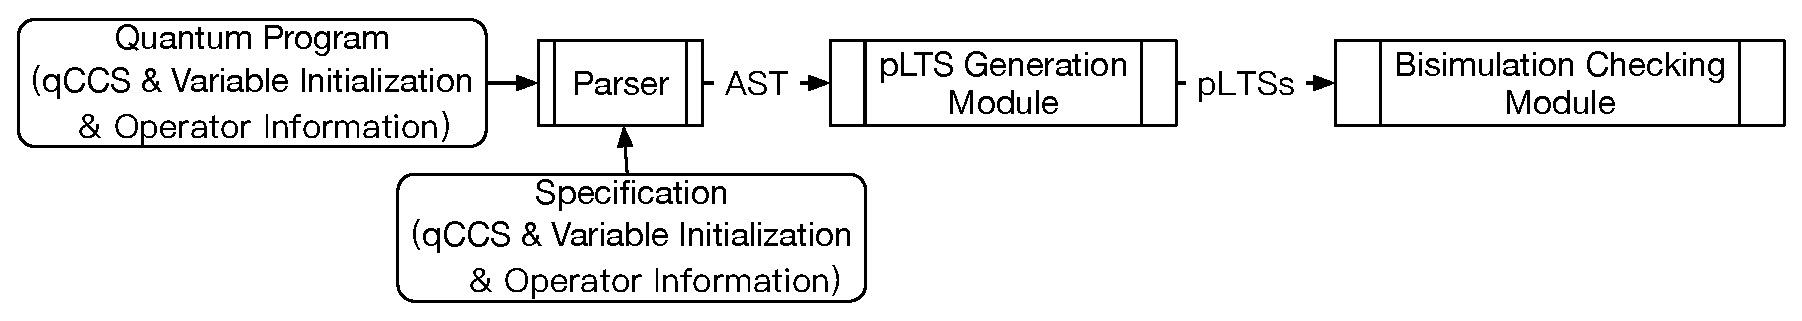
\includegraphics[width=\textwidth]{images/architecture.eps}
\caption{Verification workflow.}
\label{fig:arch}
\end{figure}
\subsection{Examples: Quantum Communication Protocols}
\subsubsection{Super-dense Coding Protocol} There are two roles $Alice$ and $Bob$. To simplify the experiment, we only consider the smallest case of the protocol, sending only one qubit. So there is totally one entanglement on two qubits in this example. Besides the Clifford operators, we use a quantum operation $Set^{\Psi}$ to present the generation of Bell state instead of the combination of the quantum gates. The operation elements of $Set^{\Psi}$ is $\{|\beta_{00}\rangle\langle00|,|\beta_{00}\rangle\langle01|,|\beta_{00}\rangle\langle10|,|\beta_{00}\rangle\langle11|\}$. The measurement is according to the computational basis $\{|00\rangle,|01\rangle,|10\rangle,|11\rangle\}$. The specification of the super-dense protocol is defined as $Bob$ sets the 2-qubit variable to the value according to the classical value he received from $Alice$.
\subsubsection{Quantum Teleportation Protocol} In this example, there are still two roles. The operators we used here is similar with the last example containing Clifford operators, $Set^{\Psi}$ and the measurement according to the computational basis. However, we need one more entanglement and one more qubit even if we just consider the smallest case. As there are more than one entanglements between these qubits, although the measurement is just applied on a part of them, it may also affect the rest qubits. We consider the final result of this protocol is presented on the third qubit, $Bob's$ qubit. It should become the same value of the first qubit. So the specification of that can be presented by applying a \textit{SWAP} operation between the first and the third qubit.
\subsubsection{BB84 Quantum Key Distribution Protocol} In BB84 protocol, there is no entanglement at all, its method needs generating qubits on different basis and using different measurement method without any contacts in advance with the other side. If someone tries intercepting the information, the qubits might be measured in wrong basis, it brings a possibility that $Alice$ and $Bob$ can be aware of the attack. So the protocol uses one more kind of measurement which is according to the diagonal basis $\{|+\rangle,|-\rangle\}$. In common use case, BB84 will send a sequence of the qubits while qubits will not influence each other. We consider two kinds of result of the communication. First case is that $Alice$ and $Bob$ choose the same measurement then the results they get are also the same. Another case is that they choose different measurements then the result is discarded at this time. In the specification, we get results from the same sequence instead of two result sequence separately. Considering results from both sides is always the same, this operation will not bring any difference.
\subsubsection{BB84 Protocol with an Eavesdropper} This example is an extension of the BB84 example, supposing there is an eavesdropper attending into the communication. There have three roles and the new role $Eve$ also randomly choose the measurement just as what $Alice$ and $Bob$ do. The specification is also similar with the one without an eavesdropper. It is possible that the eavesdropper will be recognized. It is a new result of the program. We conclude these results into three messages: emitting through the channel $alarm$ as the measurement methods are not matched; emitting through the channel $fail$ as the measurement methods are matched while the eavesdropping is recognized; normal emitting as the communication finished without recognizing the eavesdropper.
\subsection{Experimental Results}
We conducted experiments on those quantum communication protocols, and improved our input program according to the experiment results. The results were obtained on a macOS machine with an Intel Core i7 2.5 GHz processor and 16GB of RAM.
\subsubsection{Experimental Results and Improvement}Table~\ref{tab:result} provides a summary of our experimental results over those four examples. In each case, we report the bisimilarity, the number of non-bisimilar states pair in $N$ and the runtime of our checking algorithm.

We verify the super-dense coding with two different initial valuations of variable $x$ in the first two lines. In the case $x=1$, we can check that protocol and its specification are bisimilar. However, in the case $x=5$, when none of the four branches is chosen, they are not bisimilar because of the different length of the trace. The result shows that the program misses the solution for the valuation out of the expected scale. We improve the program through adding a new branch solving all the unexpected value. The result of the improved program is presented on the third line. 

Another example brings a non-bisimilarity is on the sixth line of the table, the BB84 protocol considering the eavesdropper. $Alice$ and $Bob$ will make an alert if their measurement methods are not matched. The parallelism between the final test process and them leads to the process continues behaving some actions. That is not what the specification exactly describes. To improve this program, we modify the behavior, move the alert to the test process. $Alice$ and $Bob$ only send messages when they find they use different measurements. As a result, on the last line of the table, we find the program is bisimilar with the specification.
\subsubsection{Discussion}Not all the cases of Table~\ref{tab:result} present the size of the non-bisimilar states set $N$, as the checking algorithm has terminated in advance. To ensure the bisimilarity between program with a large set of states and its specification requires much more time, over 24 times of the runtime of checking non-bisimilarity. However, the runtime of finding two pLTSs are non-bisimilar is not that long enables us to try making improvement in an acceptable time waiting feedback.
\begin{table}[h]
\centering
\begin{tabular}{@{}m{0pt}@{}
                >{\centering\arraybackslash}m{3.5cm}
                |>{\centering\arraybackslash}m{2cm}
                |>{\centering\arraybackslash}m{2cm}
                |>{\centering\arraybackslash}m{1.5cm}
                |>{\centering\arraybackslash}m{2cm}}
\hline
\rule{0pt}{5mm}&\textbf{Program} & \textbf{Variables} & \textbf{Bisimilarity} & \textbf{Size of $N$} & \textbf{Runtime}(s) \\
\hline
\hline
\rule{0pt}{12mm}&Super-dense coding 1 & \tabincell{c}{$q1=|0\rangle$\\$q2=|0\rangle$\\$x=1$} & Yes & 0 & 2.2 \\
\hline
\rule{0pt}{12mm}&Super-dense coding 2 & \tabincell{c}{$q1=|0\rangle$\\$q2=|0\rangle$\\$x=5$} & No & - & 2.2 \\
\hline
\rule{0pt}{12mm}&Super-dense coding (modified) & \tabincell{c}{$q1=|0\rangle$\\$q2=|0\rangle$\\$x=5$} & Yes & 0 & 2.5 \\
\hline
\rule{0pt}{12mm}&Teleportation & \tabincell{c}{$q1=|1\rangle$\\$q2=|0\rangle$\\$q3=|0\rangle$} & Yes & 0 & 2.7 \\
\hline
\rule{0pt}{10mm}&BB84 & \tabincell{c}{$q1=|0\rangle$\\$q2=|0\rangle$} & Yes & 304 & 4.7 \\
\hline
\rule{0pt}{12mm}&BB84 (with eavesdropper) & \tabincell{c}{$q1=|0\rangle$\\ $q2=|0\rangle$\\$q3=|0\rangle$} & No & - & 74.6 \\
\hline
\rule{0pt}{12mm}&BB84 (with eavesdropper \& modified) & \tabincell{c}{$q1=|0\rangle$\\$q2=|0\rangle$\\$q3=|0\rangle$} & Yes & 17272 & 1834 \\
\hline
\end{tabular}
\vspace{1em}
\caption{Experimental Results}\label{tab:result}  
\end{table}

\section{Conclusion and Future Works}


% ---- Bibliography ----
%
% BibTeX users should specify bibliography style 'splncs04'.
% References will then be sorted and formatted in the correct style.
%
% \bibliographystyle{splncs04}
% \bibliography{mybibliography}
%
\begin{thebibliography}{8}
\bibitem{TOCL2014}
Feng, Y., Deng, Y., Ying, M.: Symbolic Bisimulation for Quantum Processes. ACM Trans. Comput. Log. \textbf{15}(2), 14:1--14:32 (2014)


\bibitem{ref_article1}
Author, F.: Article title. Journal \textbf{2}(5), 99--110 (2016)

\bibitem{ref_lncs1}
Author, F., Author, S.: Title of a proceedings paper. In: Editor,
F., Editor, S. (eds.) CONFERENCE 2016, LNCS, vol. 9999, pp. 1--13.
Springer, Heidelberg (2016). \doi{10.10007/1234567890}

\bibitem{ref_book1}
Author, F., Author, S., Author, T.: Book title. 2nd edn. Publisher,
Location (1999)

\bibitem{ref_proc1}
Author, A.-B.: Contribution title. In: 9th International Proceedings
on Proceedings, pp. 1--2. Publisher, Location (2010)

\bibitem{ref_url1}
LNCS Homepage, \url{http://www.springer.com/lncs}. Last accessed 4
Oct 2017
\end{thebibliography}
\end{document}